
\chapter{Introduction}
\label{cha:introduction}

\section{Motivation}

\subsection{Context}

Mobile communication have shaped how people interact with each other in modern societies. Therefore, it is valid to state that mobile networks are fundamental building blocks for modern lifestyles. Usually, its infrastructure underlies silent and unnoticed. Nonetheless, when they stop working as expected, unpleasant situations, and even chaotic ones, can happen.

Usually, the most visual element of mobile networks for the common eye is the antenna towers. Although, there are several more components, both hardware and software, that enable communications as we know them.      

\begin{figure}[H]
	\centering
	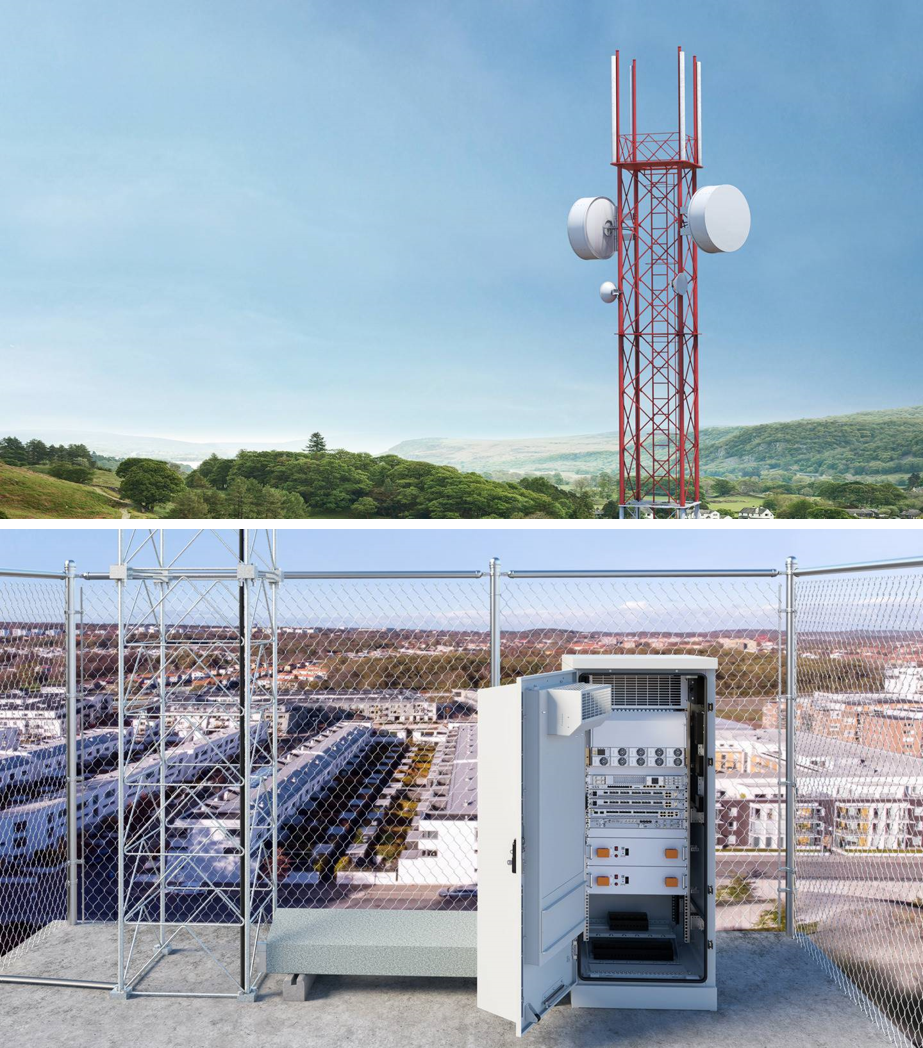
\includegraphics[width=0.42\linewidth]{figures/RBS_insfrastucture.png}
	\caption[RBS infrastructure]{RBS infrastructure. All rights belong to Ericsson}
	\label{fig:rbs_infrastucture}
\end{figure}

A \ac{rbs} is the element of telecommunication networks that receives and broadcasts electromagnetic waves to the environment in a determined area and is therefore one of the essential pieces to enable mobile communication. 

Mobile networks are geographically distributed in units called \emph{antenna site} consisting of multiple cells which comprise more than one cell --usually three--. Depending on its technology, it will vary its components and the architecture in which they are connected, as shown in Figure \ref{fig:rans}. Nonetheless, the main principles stand. 

\begin{figure}[H]
	\centering
	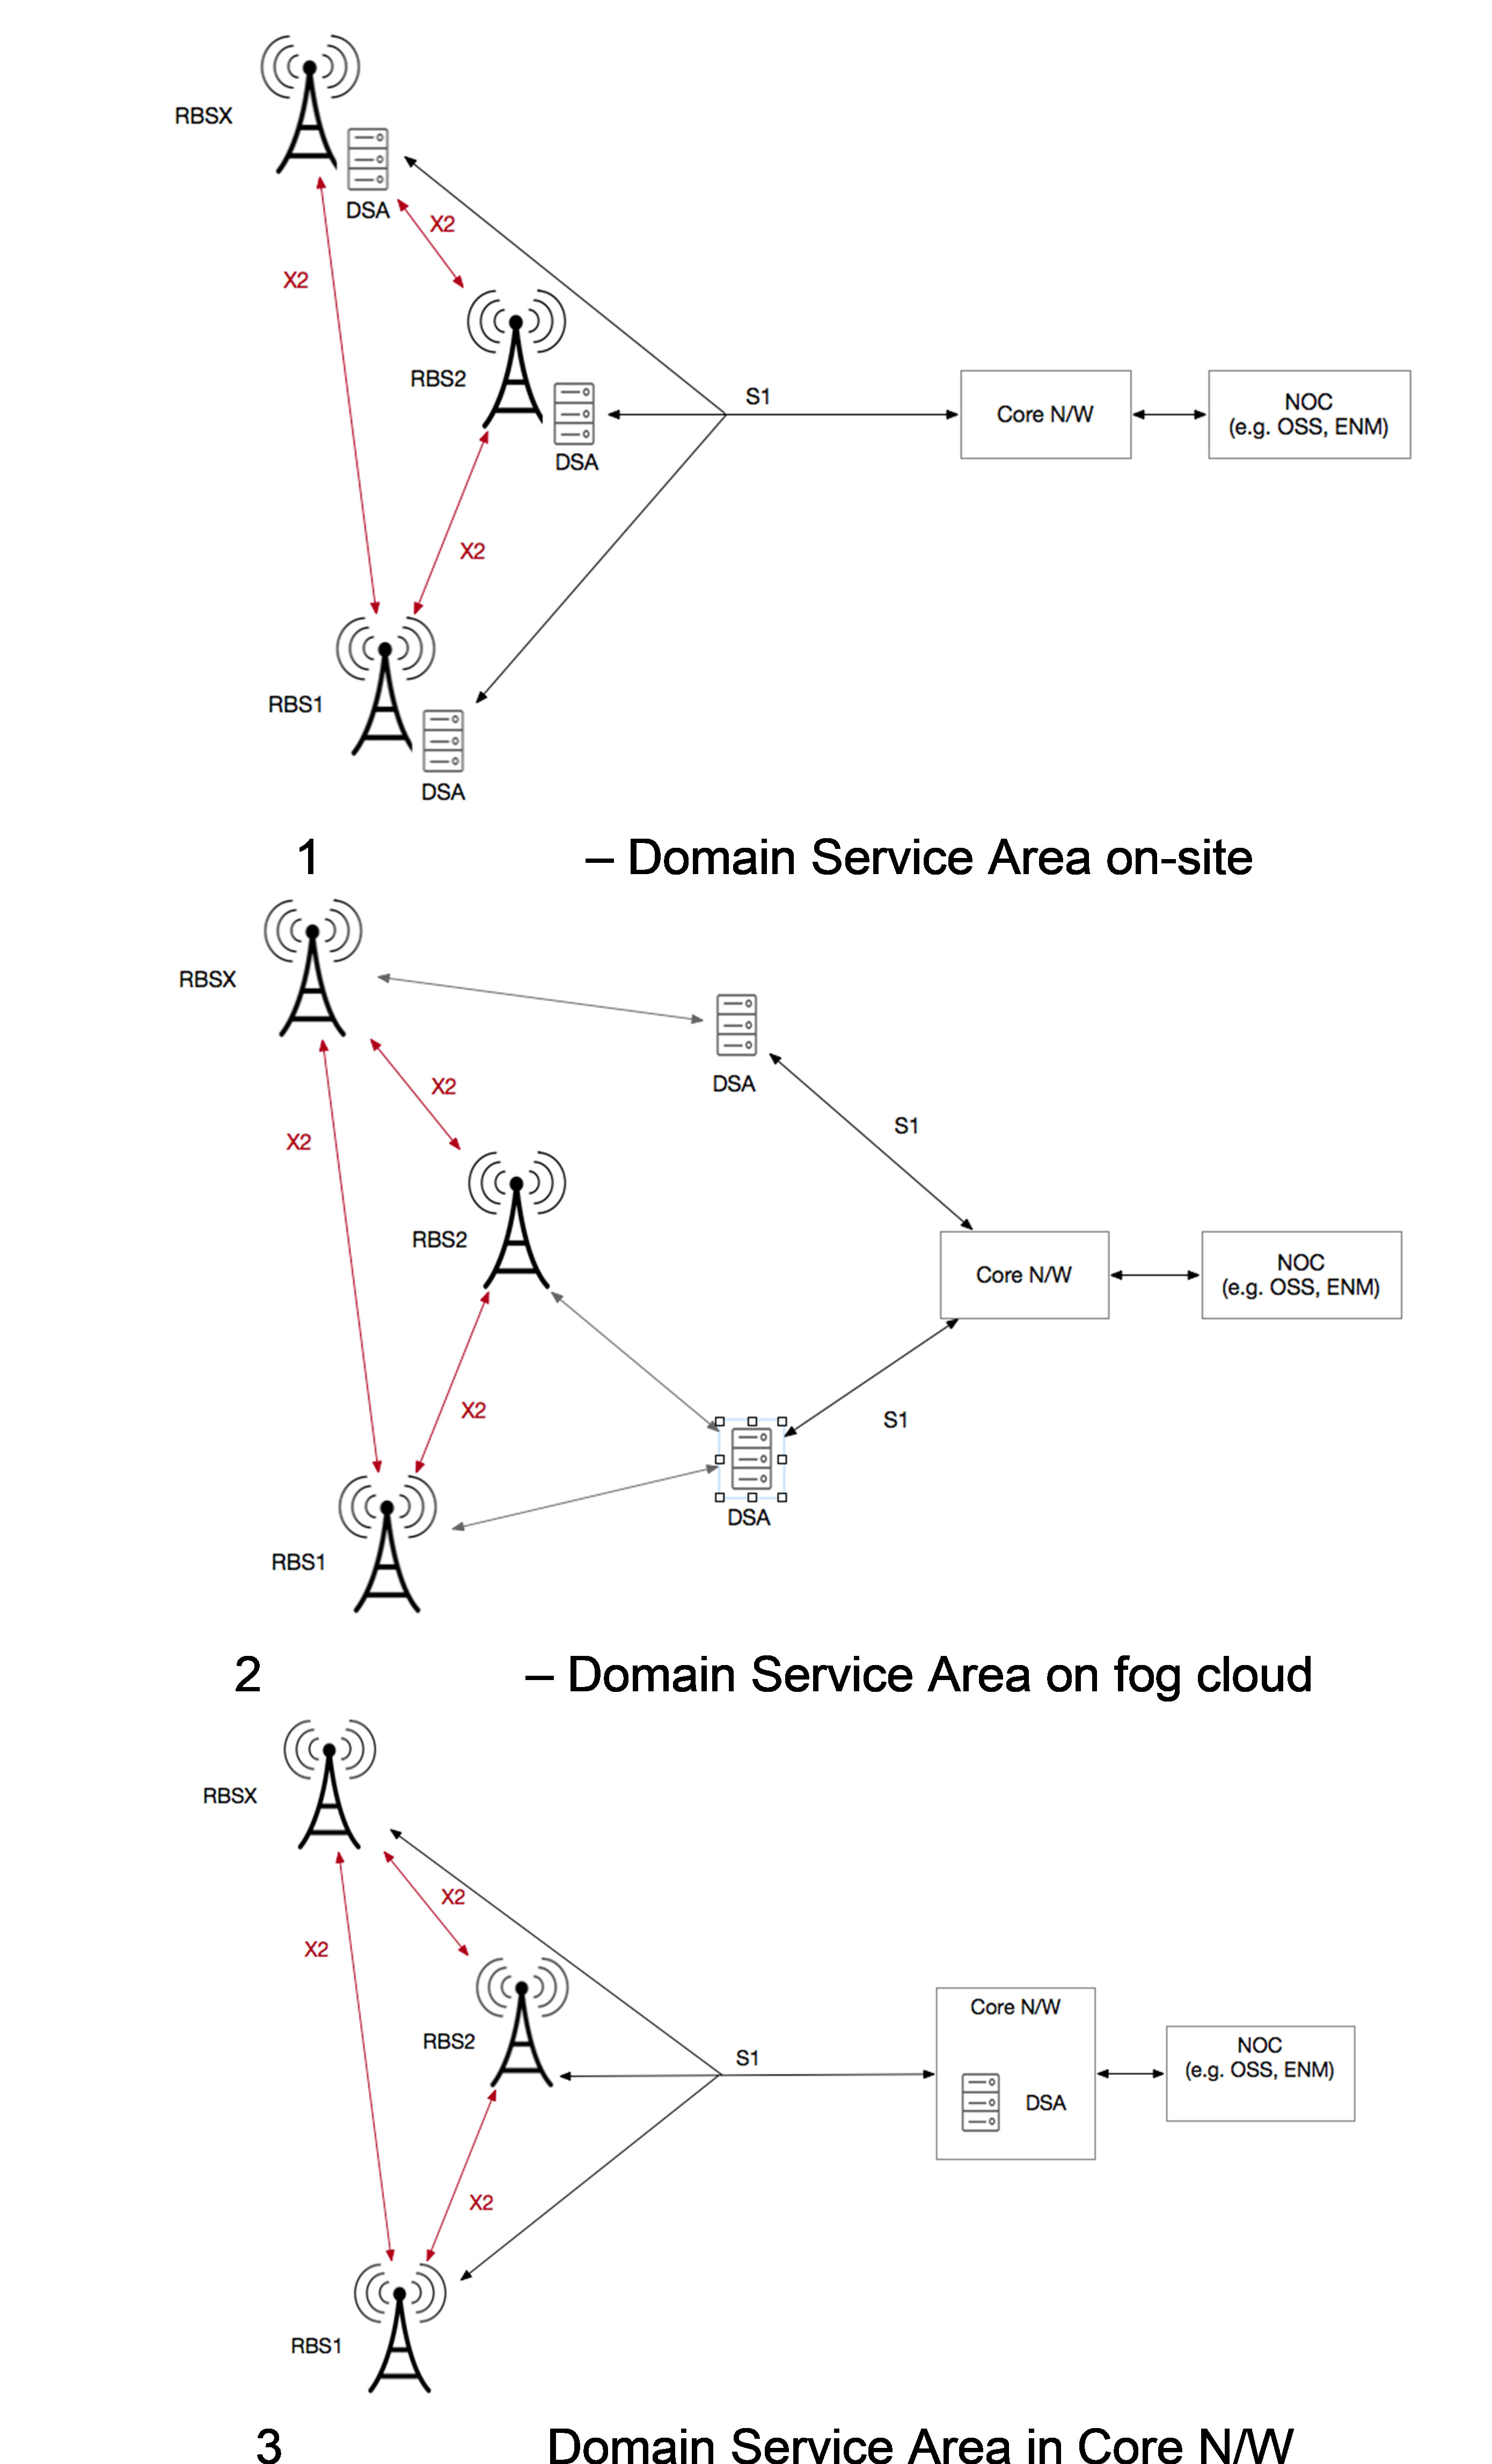
\includegraphics[height=0.9\linewidth]{figures/RANs.png}
	\caption{Different Radio Access Networks architectures}
	\label{fig:rans}
\end{figure}

In present \acp{rbs}, in case of any hardware fault,  an alarm is triggered and sent to the fault management system (reporting system) and informed to the \ac{oss} in order to be processed and handled by the \ac{noc}. Engineers in the \ac{noc} should raise a request to send the field workforce to replace the faulty unit based on the alarm data.

The reality is that not all of the alarms affect the radio performance or cause degradation of the radio traffic, which implies that there is no urgency in sending service personnel to the \ac{rbs} site until its operational continuity is at risk. 

Setting the right time for sending field workers to the \ac{rbs} to replace hardware, which sometimes might be located in very isolated or hard to reach locations,  would positively affect the maintenance and operational costs for the \acp{mno}.

%As a Statistics and Machine Learning research, the current work does not aim to provide deep knowledge on telecommunications networks. Thus, some communications concepts will not be thoroughly developed, which does not imply any lack of statistical research rigorousness.

In this thesis, the focus will be on the statistics and machine learning research rather than on communication networks development. Thus, some communications concepts will not be thoroughly developed.

\subsection{PSU alarms and power headroom}

The \acf{psu} powers the entire \ac{rbs}. Nonetheless, usually, one station may contain several \acp{psu} for operational robustness in case of faults, as shown in Figure \ref{fig:powerinfrastucture}. This redundancy implies that when an alarm is received from a \ac{psu}, sometimes, there is no need for an immediate replacement of the faulty \ac{psu} hardware since the \ac{rbs} has still enough power available to continue its operation without blackout risk. 

\begin{figure}[H]
	\centering
	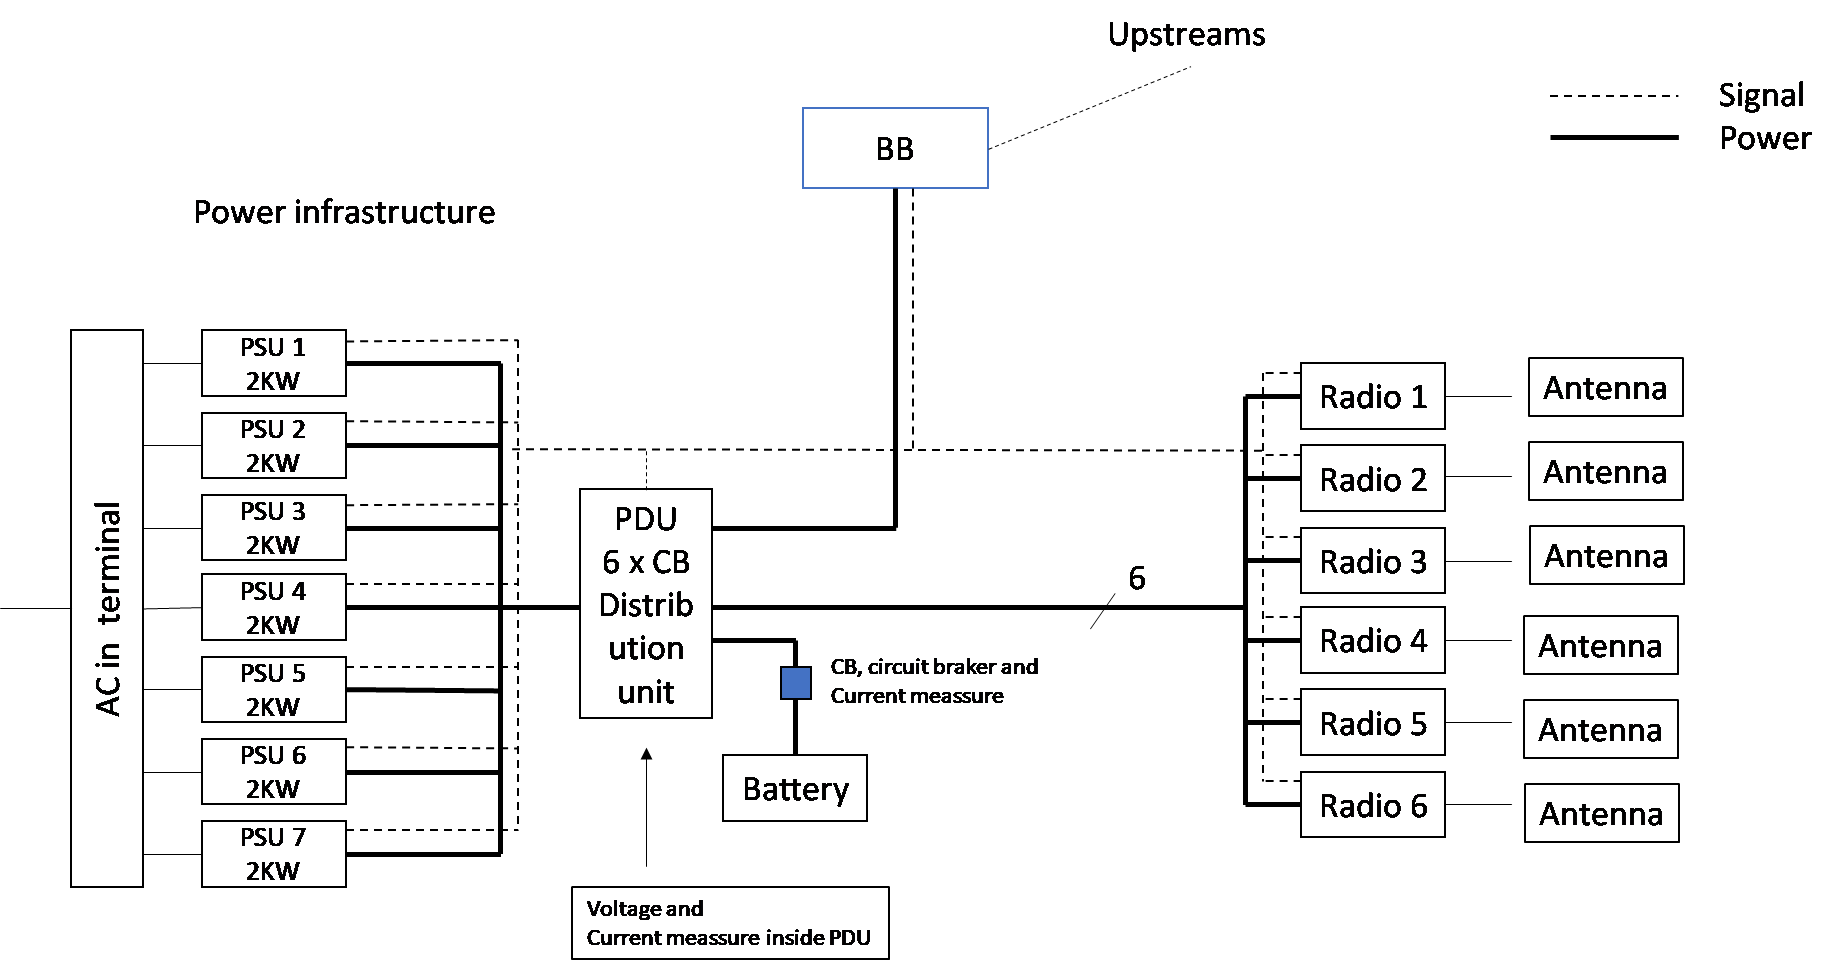
\includegraphics[width=0.95\linewidth]{figures/power_infrastucture}
	\caption[Example of a power infrastructure in an \ac{rbs}]{Example of a power infrastructure in an \ac{rbs}\protect\footnotemark}
	\label{fig:powerinfrastucture}
\end{figure}

\footnotetext{This is a general overview of the power infrastructure in an \ac{rbs}, i.e., each station may differ from others depending on how the ad-hoc solution has been designed}

Other components to note to better understand the features are the \ac{pdu} which is the unit that manages the power of the system and distributes it according to different operational scenarios. The \acp{ru} are, as its name explains, the units in which the power is converted into electromagnetic waves modulated to carry information and then uses the antennas to broadcast them into the ambient. Last but not least are the power lines, which are not a unit themselves, but interconnects the units so the \ac{rbs} itself could work as a system. The power lines are the veins that carry the energy to all the elements within the system. Nonetheless, they are not ideal, and power gets dissipated along them. The longer the lines are, the higher the losses.


Added to the power surplus given by redundant \acp{psu}, there is also the fact that not all the available power is used all the time because the radio traffic has a clear seasonal component as shown in Figure \ref{fig:connectionstwoweeks}. Thus, the \acp{ru} are not constantly transmitting at their maximum capacity.


\begin{figure}[H]
	\centering
	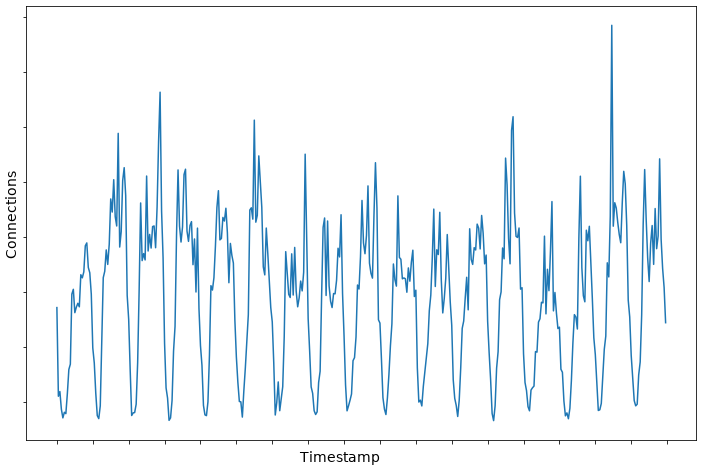
\includegraphics[width=0.8\linewidth]{figures/connections_two_weeks}
	\caption{Example of variation of a number of connections in a \ac{rbs}}
	\label{fig:connectionstwoweeks}
\end{figure}

Given this surplus in energy, the PSU \emph{power headroom}\footnote{This shall not be confused with the power headroom defined in 3GPP. We have used the same \emph{headroom} terminology so communication engineers could easily understand its main concept. But is has to be emphasised that this is related to \ac{psu} power and not to Radio power.} $P_h$ can be defined as the difference between the power consumption $P_{cons}$ and the maximum available power $P_{max}$.

\begin{equation}\label{eq:phdroom}
	P_h = P_{max} - P_{cons}
\end{equation}

Where $P_{cons}$ can be understood as \emph{the consumed power seen from the \ac{psu}} \cite{muhammad2010uplink,procedures20123gpp}, which will comprise the \acp{ru} power consumption, static power consumption, cooling system consumption, the losses in the lines, etc. For simplicity, this definition will not be developed in-depth.

In Figure \ref{fig:powerheadroom} it is shown how the amount of \acp{psu} is related to the power headroom and how a decrease in the amount of working \acp{psu} would diminish the power headroom value but still give a reasonable operational margin.   

\begin{figure}[H]
	\centering
	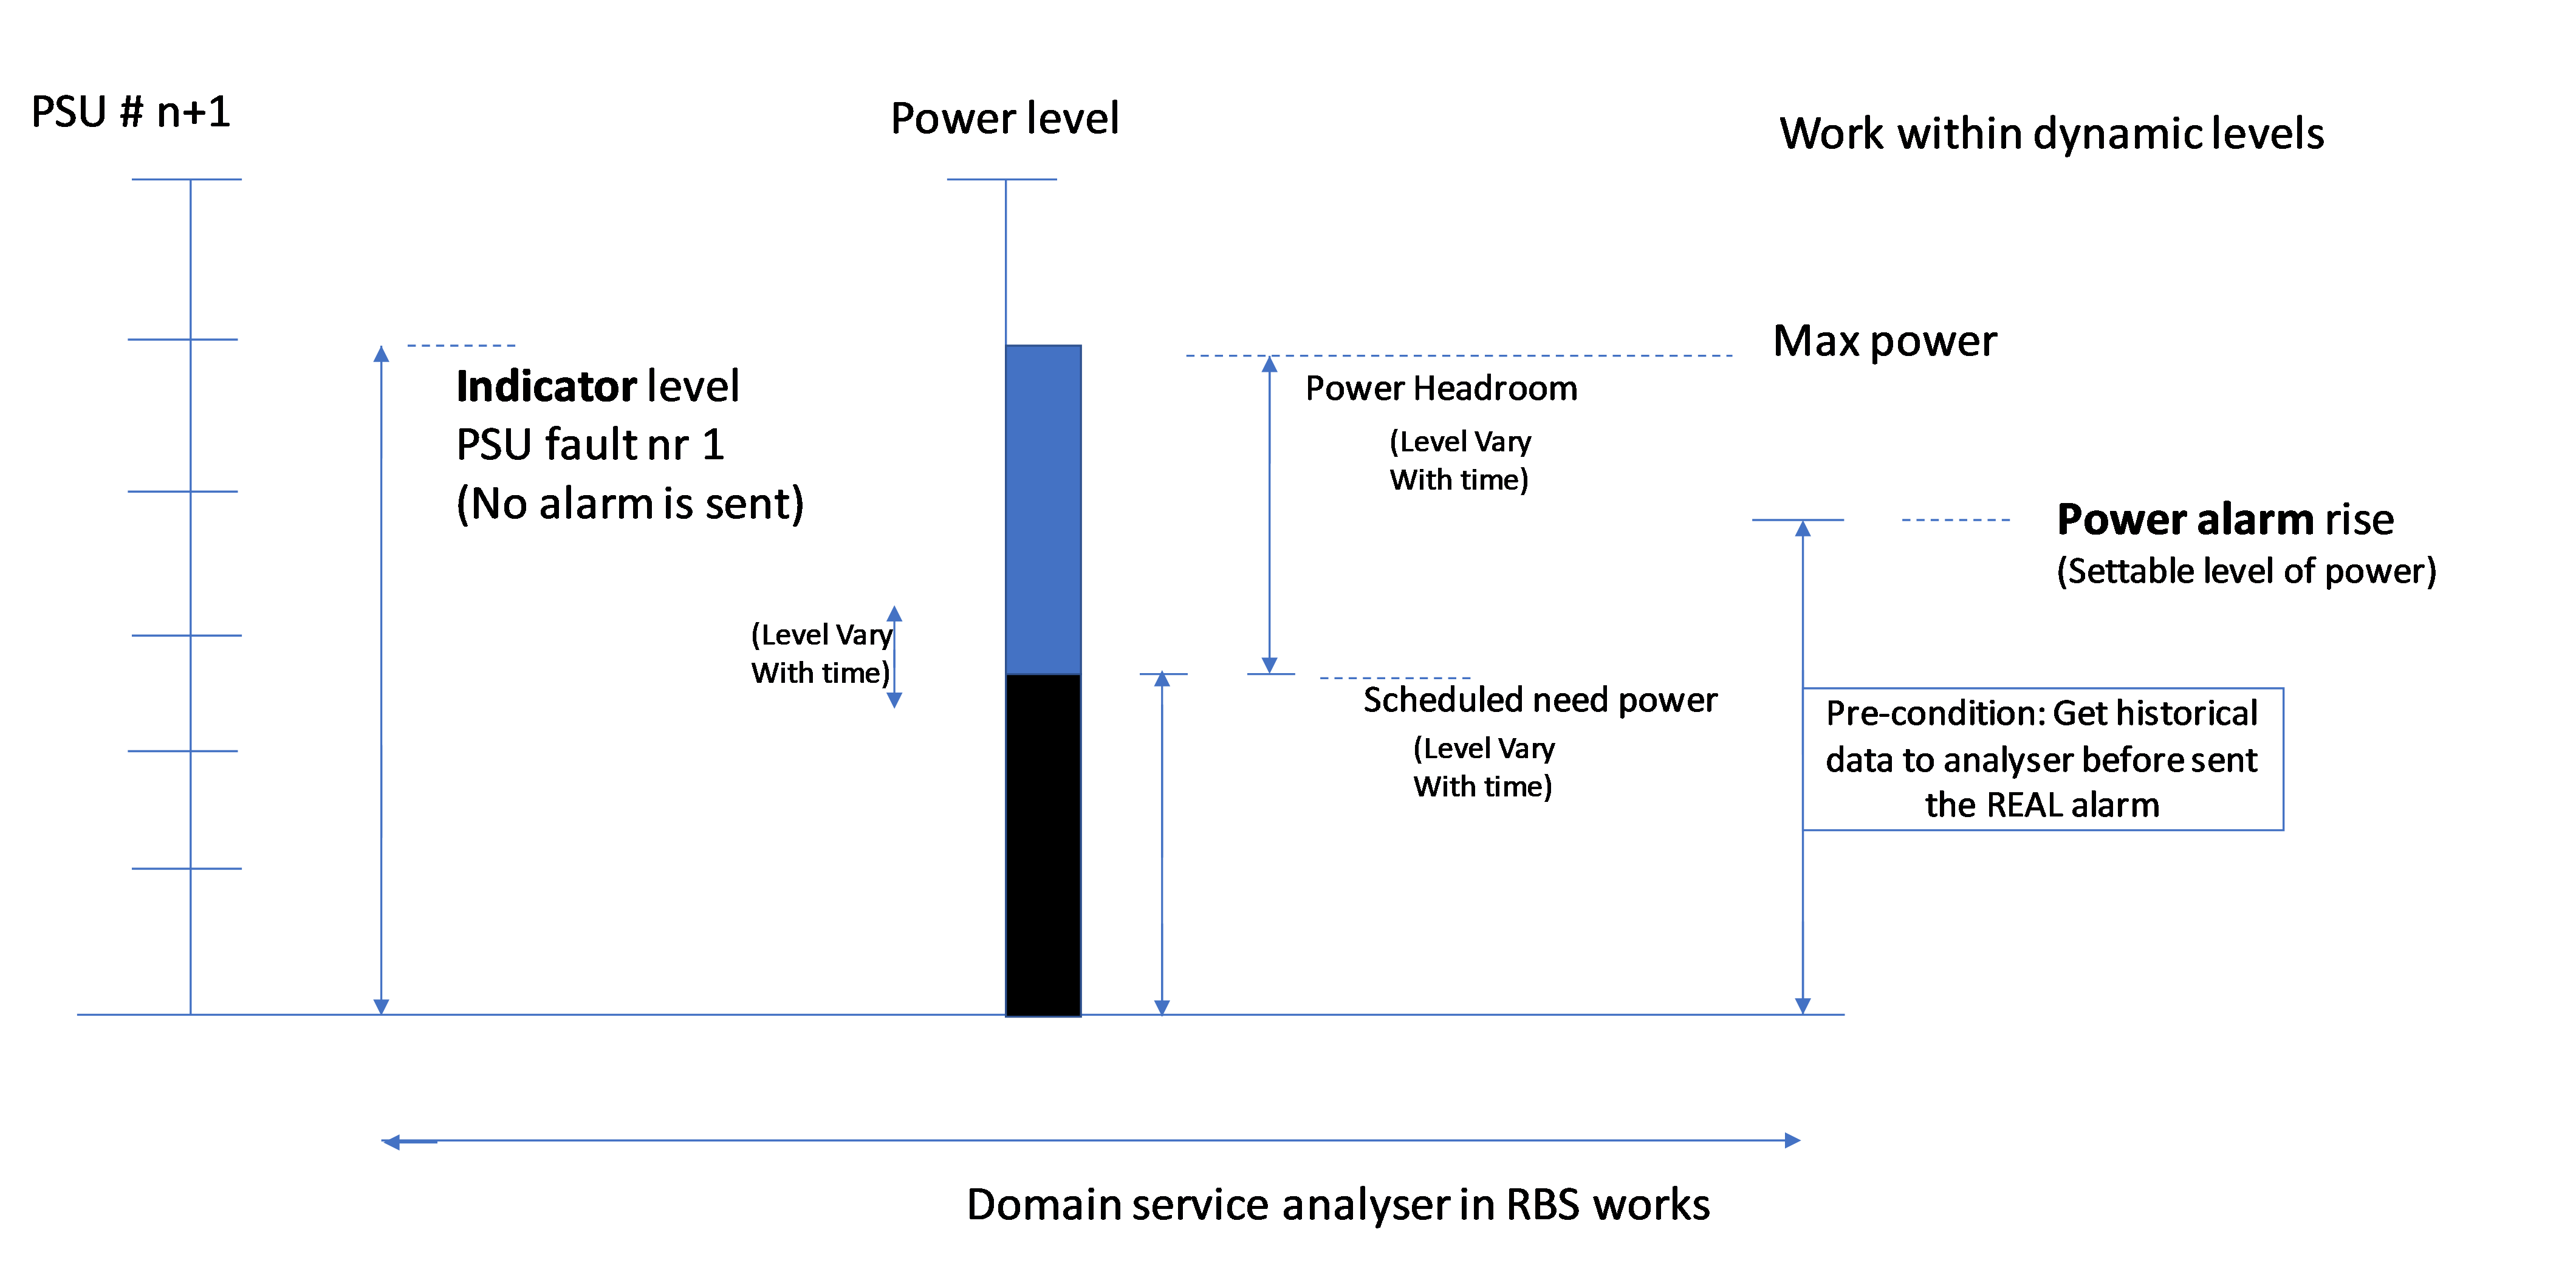
\includegraphics[width=0.95\linewidth]{figures/power_headroom}
	\caption[Power headroom]{Power headroom example}
	\label{fig:powerheadroom} 
\end{figure}



\pagebreak
\section{State-of-the-art}

The research on power consumption in \acp{rbs} is not a new topic in the communication community and it can be seen from two different research perspectives. The first stands from a modelling point of view. It can have a top-to-down approach \cite{power_modeling}, i.e., focusing on the consumption first, and based on them, describe the system. Alternatively, there is a bottom-up perspective, in which the overall power consumption of the system is described by the consumption of each independent building block depending on their different operational modes \cite{power_detailed}\footnote{ This study considers: power amplifier, analogue frontend, digital baseband, digital control and power system}. Both have in common that they are descriptive in nature and have constrained their data to pure hardware technologies and their power characteristics. Their primary purpose has been modelling and simulation of power consumption in communication networks.


The second perspective uses more data than just hardware descriptions. As a consequence, traffic metrics have been shown to be a fundamental covariate to explain power consumption fluctuations in \acp{rbs} \cite{powerregression}. Furthermore, STL decomposition has been applied to model the traffic load in \acp{rbs}. Then, Holt-Winter's technique \cite{winters1960forecasting} has been used to forecast its values, so the power management can adopt power-saving strategies when it is not needed to broadcast at maximum power capacity \cite{piunti40traffic}.

When it comes to power consumption forecast in domains other than telecommunication, the field has also been fruitful. Sensor network's power consumption using Markov chains \cite{achir2004power}, power consumption in data centres using LASSO, elastic-net, \ac{rf}, KNN, and \ac{mlp} \cite{deepika2020power}, coal-mining power consumption forecast using pure statistics \cite{antonenkov2017mathematic} or laser-melting processes using linear regression \cite{lv2020novel}, to mention some.  

Furthermore, forecast household power demand is a very fertile domain on its own. Linear regression, decision trees, \ac{rf}, \ac{svr} and \ac{mlp} have been applied to predict the demand in northern Morocco \cite{morocco} finding that \ac{mlp} performs better than the others. \ac{lstm} networks have been applied to learn household consumption and have been compared against \ac{gbt} and \ac{svr} approaches finding that the \ac{lstm} model, which they have called \emph{PowerLSTM}, outperforms the others\cite{powerlstm}. A novel \ac{eennp} method is proposed in \cite{ai2019household} and applied to power consumption in western Norway. 

The well-used Holt-Winters model has been compared against Facebook's Prophet model in long-range power loads forecast in Kuwait, reaching a $\text{MAPE}\sim2\%$ for a prediction horizon of 720 days. Their predictions robustness has been tested by injecting Gaussian noise in different intensities at a fixed (unspecified) forecasting horizon, concluding that Prophet can perform robust power demand predictions while obtaining $R^2=0.96$ at a noise intensity of $80\%$ \cite{almazrouee2020long}. In the same direction, it has been shown that Prophet performs better than ARIMA models for a long-range of 30 days on power demand prediction using external environmental regressors in an airport in Belgium \cite{chadalavada2020electricity}. In both studies, Prophet's weekly seasonal component is used to recommend the most suitable day of the week to perform maintenance related to power consumption.  

Furthermore, in \cite{jiang2021clothing}, the potential of Prophet for long-range predictions has been shown by extending it to work together with a \ac{gru} as an attention layer plus a \ac{critic} node to weigh both predictions optimally. For a prediction horizon of $\sim6$ months, the proposed architecture show a $\text{MAE}=8.5$ against $10.1$ and $20.1$ from Prophet on its own and ARIMA, respectively.  

%Thus, the robustness of the predictions made by Prophet models for long-range time horizons makes it an interesting alternative to be applied in the telecom domain. Additionally, it has shown to perform better than standard methods in other fields, which are also highly related to human behaviours. No publication has been found doing so during the research.

Thus, the robustness of the predictions made by Prophet models for long-range time horizons in addition to that it has shown to perform better than standard methods in other fields, which are also highly related to human behaviours, makes it an interesting alternative to be applied in the telecom domain. No publication has been found doing so during the research.



\pagebreak
\section{Aim}
\label{sec:aim}

The following work aim to develop a statistical or machine learning method that reports an alarm if, and only if, the power headroom in a \ac{rbs} will reach unsafe operational levels based on installed power capacity and power consumption forecasts. 

Based on state-of-the-art findings, exploring Prophet's capabilities to also endow of long-range robustness the proposed solution.


\section{Research questions}
\label{sec:research-questions}

\begin{enumerate}
	\item What is the best way to handle real-world telecommunication and power time series to provide useful structures to mine and learn from them?
	\item What are suitable forecast techniques to predict power utilisation in an \ac{rbs}?
	\item Given the power forecast, what are suitable criteria to raise alarms, if and only if, the \ac{rbs} operational continuity is at risk?
\end{enumerate}

\section{Delimitations}
\label{sec:delimitations}


Even though one of the overall goals of the work has been reducing operational costs for \acp{mno}, this has been done without considering the logistics under maintenance, or stock constraints of hardware replacement stock or even \ac{rbs} geographical location. Therefore, the only factor of operational costs this work tries to optimise is \emph{when} a hardware replacement alarm is raised.



